\documentclass[a4paper,10pt]{article}
\usepackage[margin=0.75in]{geometry}
\usepackage{graphicx}
\usepackage{parskip}
\usepackage{caption}
\usepackage{float}
\usepackage{multicol}
\usepackage{fancyhdr}
\usepackage{titlesec}
\usepackage{lmodern}
\usepackage{qrcode}
\pagestyle{fancy}

\titleformat{\section}{\large\bfseries}{}{0em}{}

\fancyhead[R]{Rafferty Simms --- N0990815}

\begin{document}

\begin{center}
    {\LARGE \textbf{Gait Recognition-based Authentication for User-Independent Physical Access Control}}\\
    \vspace{0.5em}
    {\large An unobtrusive, contactless biometric authentication method using walking patterns}
\end{center}

\section*{What Is Gait Recognition?}
Gait Recognition (GR) is a biometric technique that identifies individuals based on the unique way they walk.
Unlike facial or fingerprint recognition, GR enables \textbf{passive, non-intrusive identification} — requiring active user participation or use of physical tokens.

\section*{Why Use Gait for Access Control?}
\begin{itemize}
    \item \textbf{Transparent Authentication}: Users are authenticated simply by walking past a camera.
    \item \textbf{User-Independent}: No PINs, keycards, or smartphones required.
    \item \textbf{Bias Reduction}: Less reliant on facial features; less prone to racial or lighting-related bias.
    \item \textbf{Contactless}: Ideal for hygiene-sensitive environments.
\end{itemize}

\vspace{0.5em}
\rule{\linewidth}{0.4pt}
\vspace{0.5em}

\section*{System Overview}

\vspace{0.5em}
\noindent
Movement Input → Silhouette Extraction → GEI Creation → Identity Classification → Access Decision

\begin{figure}[H]
    \centering
    \begin{minipage}[t]{0.53\textwidth}\vspace{0pt}
        \begin{minipage}[t]{0.31\textwidth}\vspace{0pt}
            \centering
            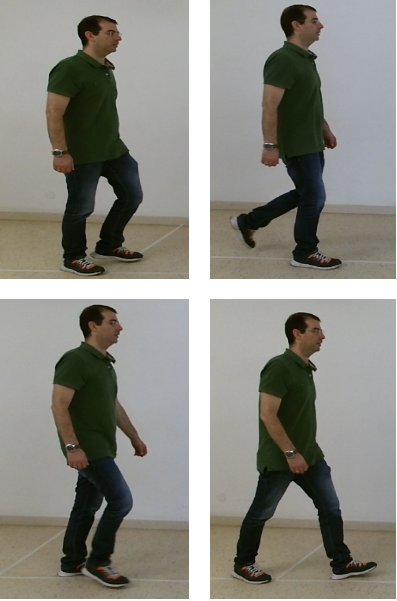
\includegraphics[width=\linewidth]{assets/gei-flow_a.png}
            \caption*{Movement}
        \end{minipage}
        \hfill
        \begin{minipage}[t]{0.31\textwidth}\vspace{0pt}
            \centering
            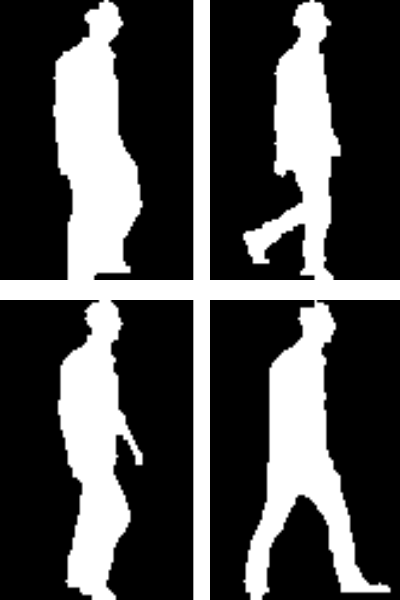
\includegraphics[width=\linewidth]{assets/gei-flow_b.png}
            \caption*{Silhouettes}
        \end{minipage}
        \hfill
        \begin{minipage}[t]{0.31\textwidth}\vspace{0pt}
            \centering
            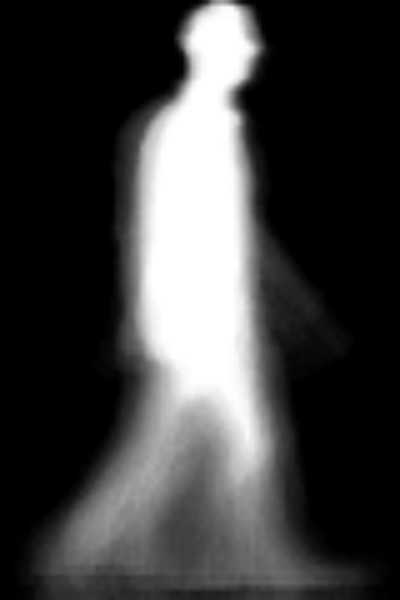
\includegraphics[width=\linewidth]{assets/gei-flow_c.png}
            \caption*{Gait Energy}
        \end{minipage}
    \end{minipage}
    \hfill
    \begin{minipage}[t]{0.42\textwidth}\vspace{0pt}
        \centering
        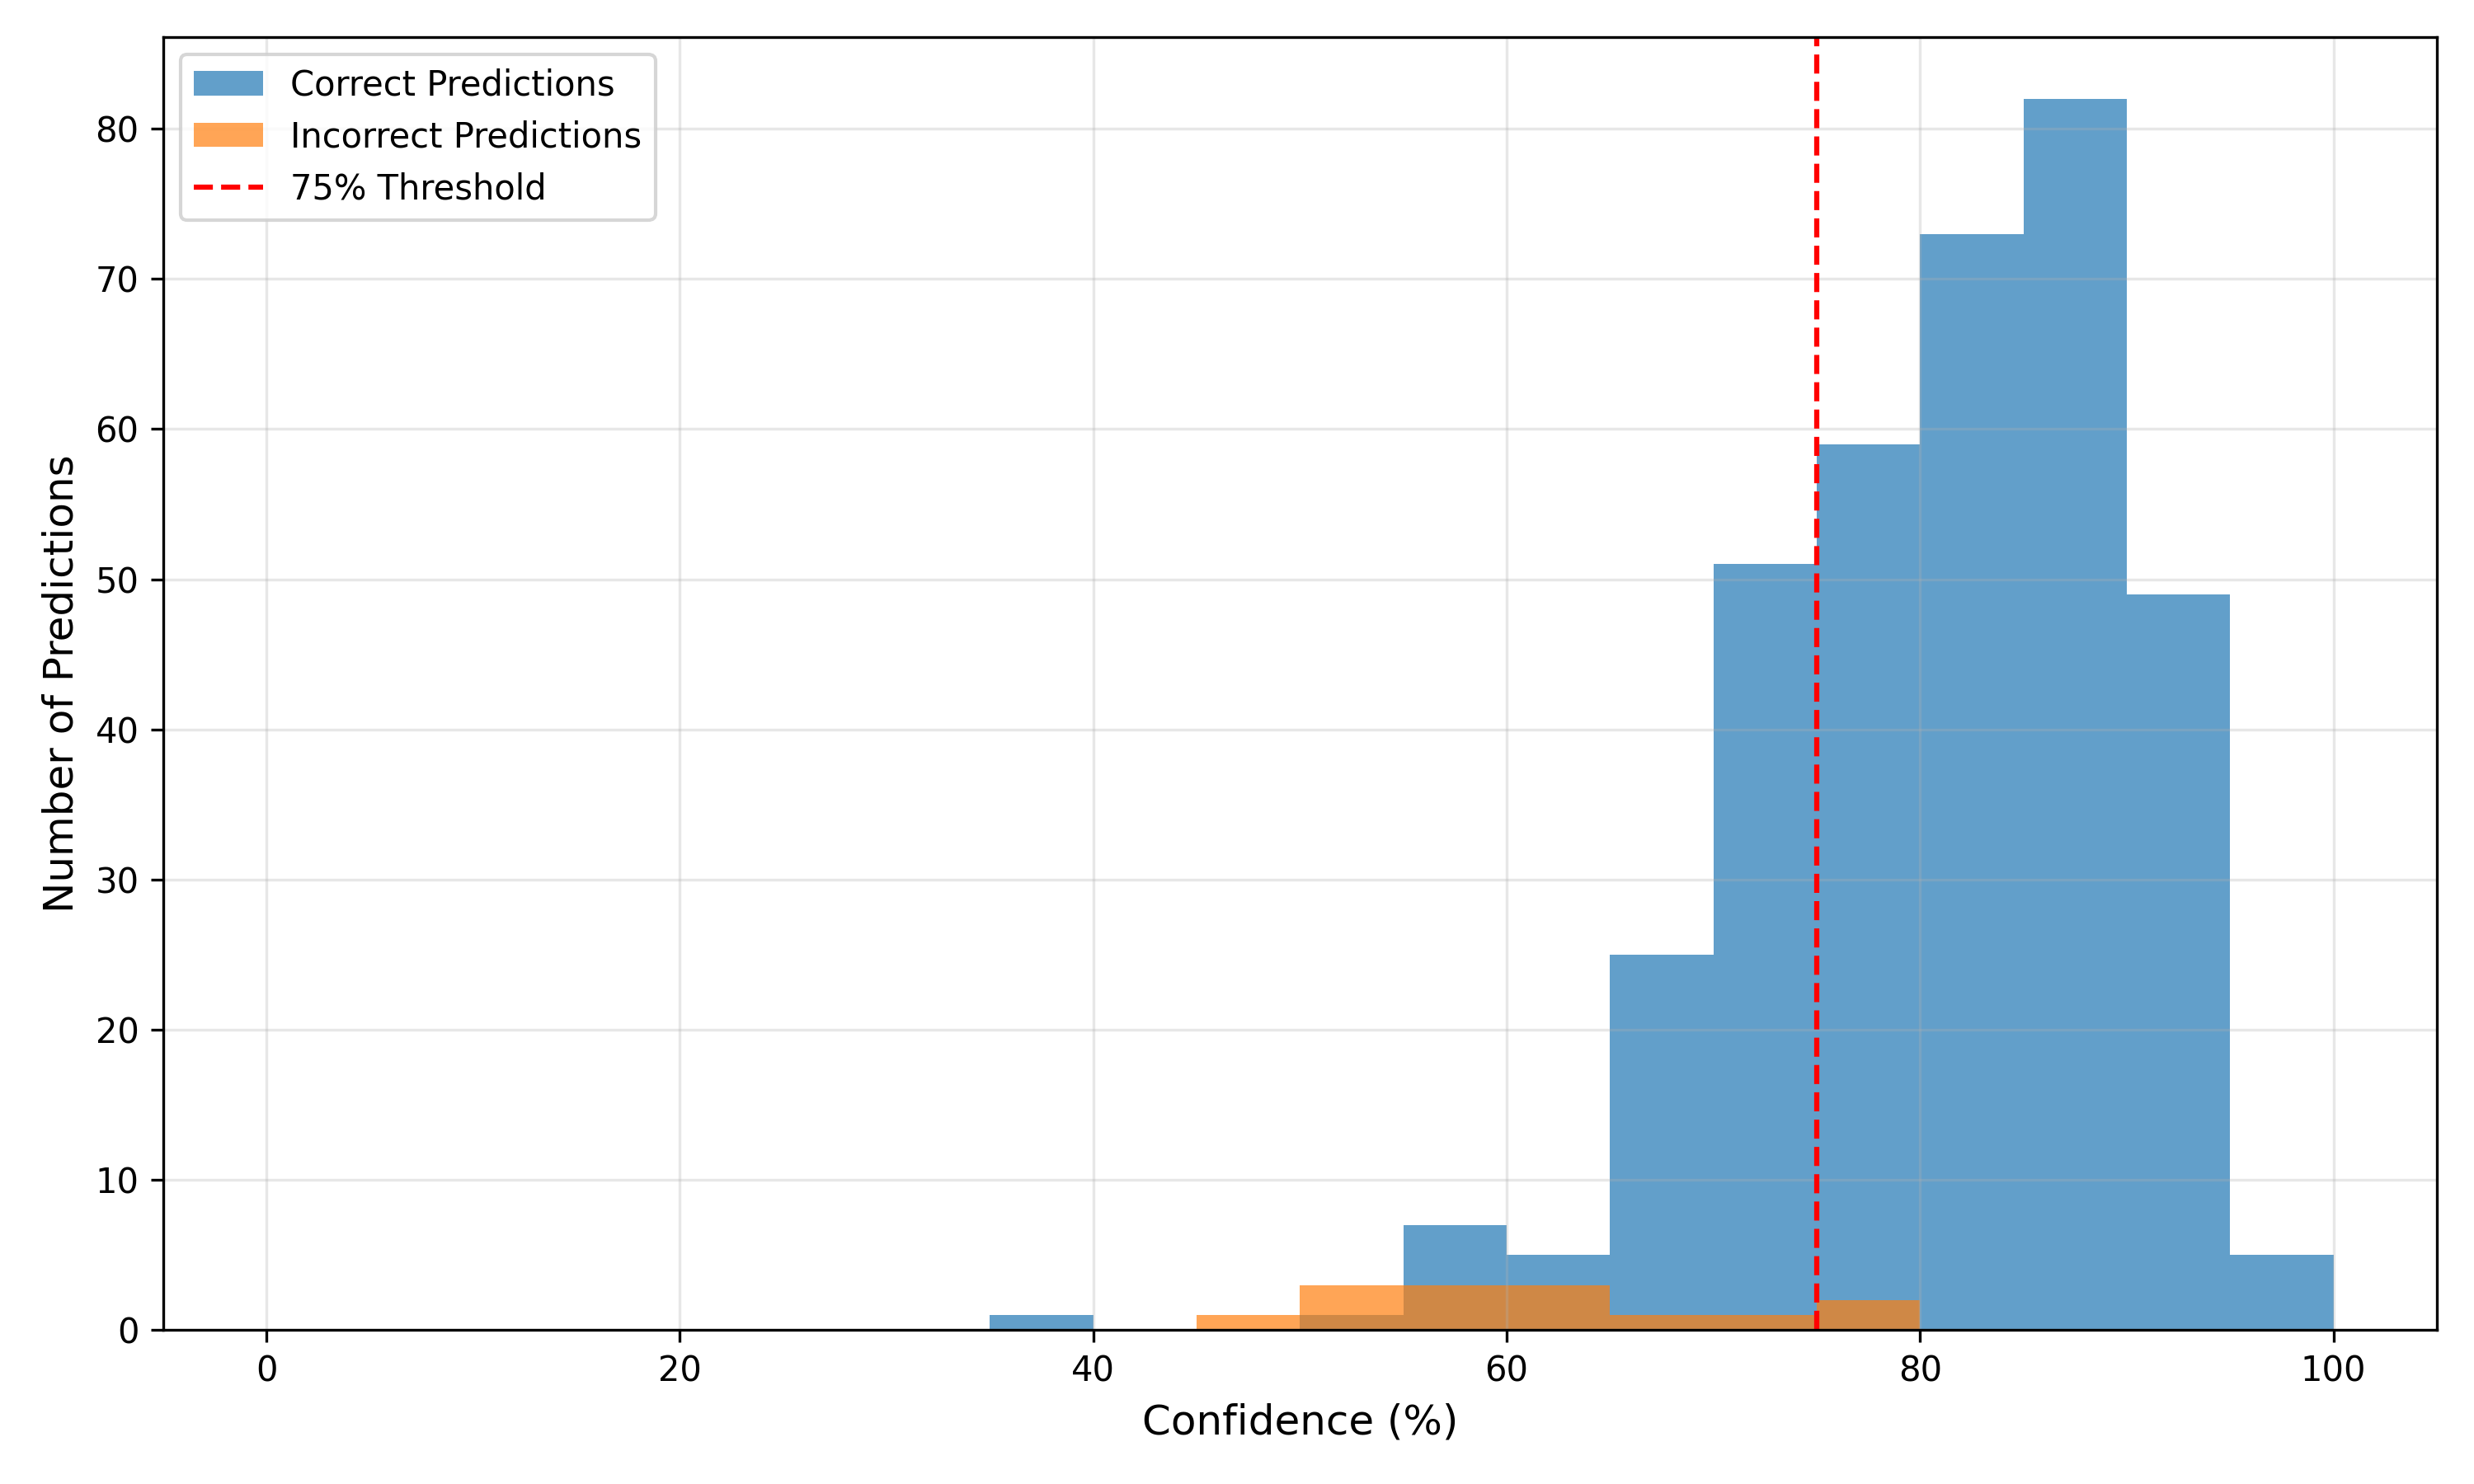
\includegraphics[width=\linewidth]{assets/gei_analysis_confidence_distribution.png}
        \captionof*{figure}{Classification Confidence Distribution}
    \end{minipage}
\end{figure}

\rule{\linewidth}{0.4pt}
\vspace{0.5em}

\noindent\begin{minipage}[t]{0.65\textwidth}\vspace{0pt}
    \small
    \section*{Highlights}
    \begin{itemize}
        \item Achieved approximately 90\% classification accuracy in testing, with 70\% of cases exceeding a 75\% confidence threshold.
        \item Supports real-time computer vision processing and manual uploads, enabling both live and asynchronous recognition via a client-server architecture.
        \item Received positive user feedback highlighting transparency and convenience; some concerns raised around surveillance implications and data privacy.
        \item Operates efficiently on low-power consumer hardware, demonstrating potential for affordable, scalable deployment.
        \item End-to-end access control logic successfully validated, including live identity classification and access rule toggling through a working web interface.
    \end{itemize}
\end{minipage}%
\hfill
\begin{minipage}[t]{0.3\textwidth}\vspace{0pt}
    \begin{center}
        \section*{LinkedIn}
        \qrcode[height=5cm]{https://www.linkedin.com/in/raffsimms/}
    \end{center}
\end{minipage}



\end{document}
